\documentclass[main.tex]{subfiles}
%\graphicspath{{\subfix{../images/}}}
\begin{document}
\begin{enumerate}[label=\textbf{\alph*)}]
    \item Houve uma melhora considerável entre o método de Euler simples para os outros dois: Euler-Cromer e Runge-Kutta. Pode-se dizer que foi uma melhora pois para um pêndulo sem amortecimento, espera-se que o movimento esteja confinado num intervalo, isto é, com uma amplitude fixa. Claramente para o primeiro método, a amplitude do movimento aumenta sem que qualquer força externa tenha sido aplicada.
    Esse problema é minimizado nos dois outros métodos, onde não é possível ver nenhuma variação na amplitude - olhando apenas para esses dois gráficos.
    \begin{center}
        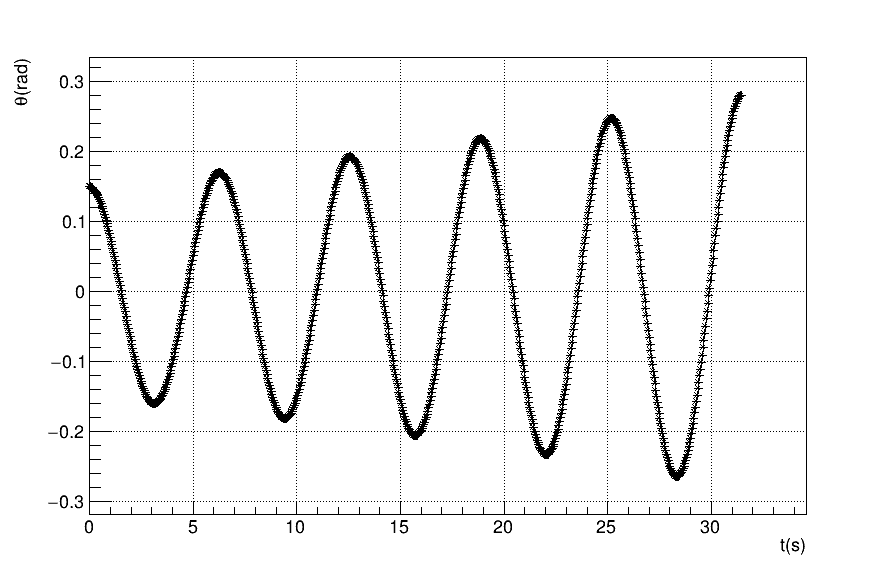
\includegraphics[scale=0.15]{../q1/plots/theta_t_euler.png}
        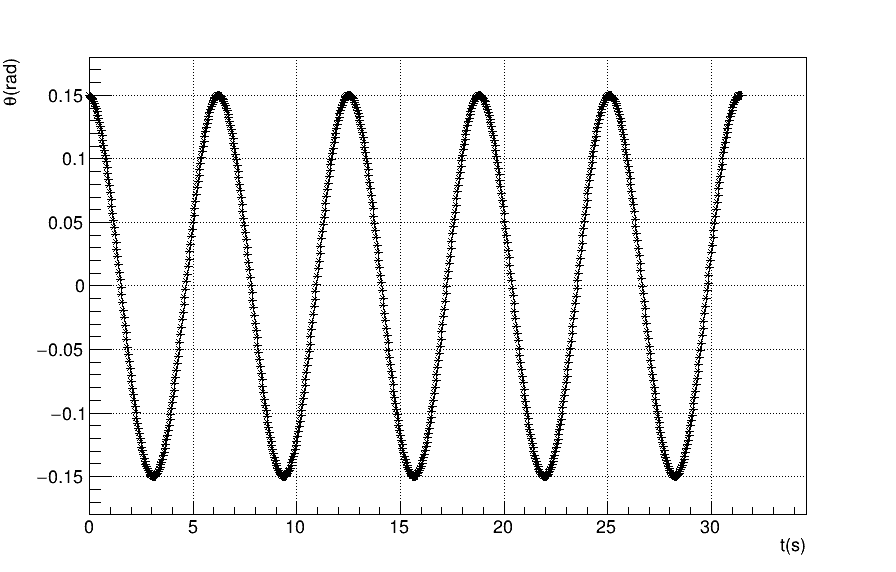
\includegraphics[scale=0.15]{../q1/plots/theta_t_ec.png}
        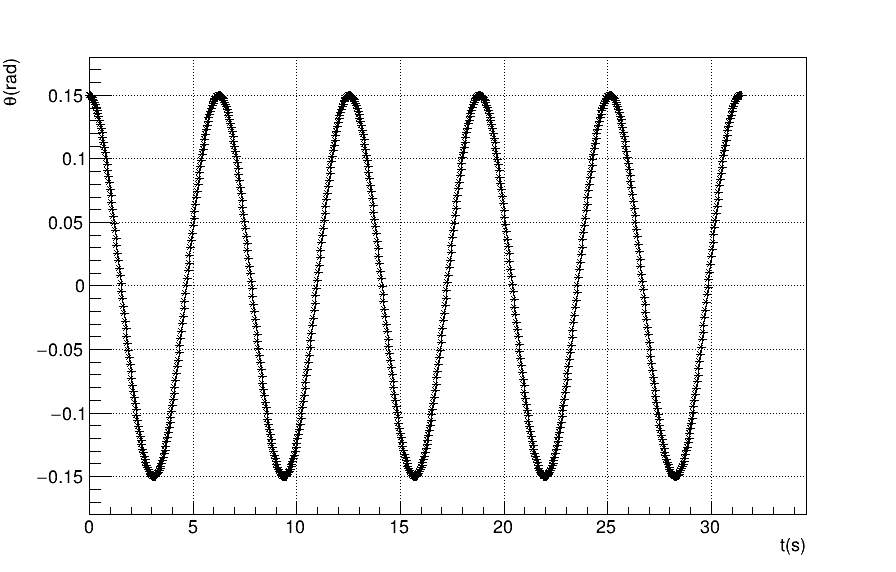
\includegraphics[scale=0.15]{../q1/plots/theta_t_RK.png}
        \captionof{figure}{Gráficos de $\theta \times t$ para os métodos de Euler simples, Euler-Crome e Runge-Kutta, respectivamente da esquerda para direita. }
    \end{center}
    \item Para o gráfico de $\omega \times t$, pode-se confirmar que o método de Euler simples mostra que pêndulo fica mais rápido a cada período, enfatizando o argumento do item (a). Já os outros dois métodos continuam não mostrando diferença aparente entre si e parecem reproduzir o movimento esperado.
    \begin{center}
        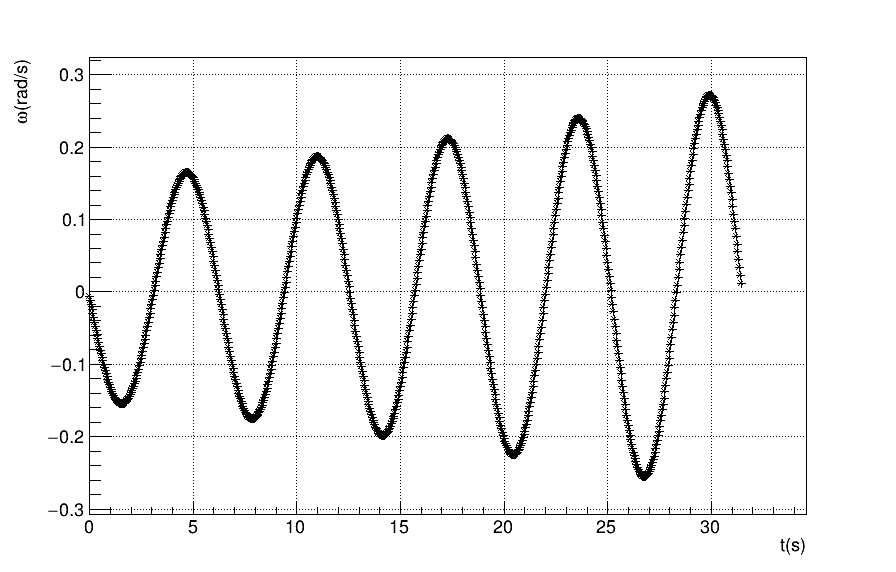
\includegraphics[scale=0.15]{../q1/plots/omega_t_euler.png}
        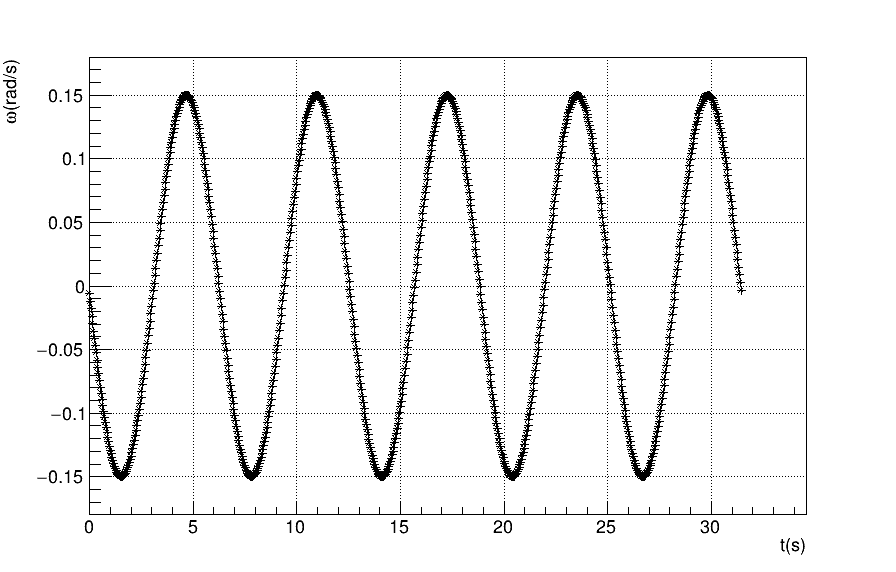
\includegraphics[scale=0.15]{../q1/plots/omega_t_ec.png}
        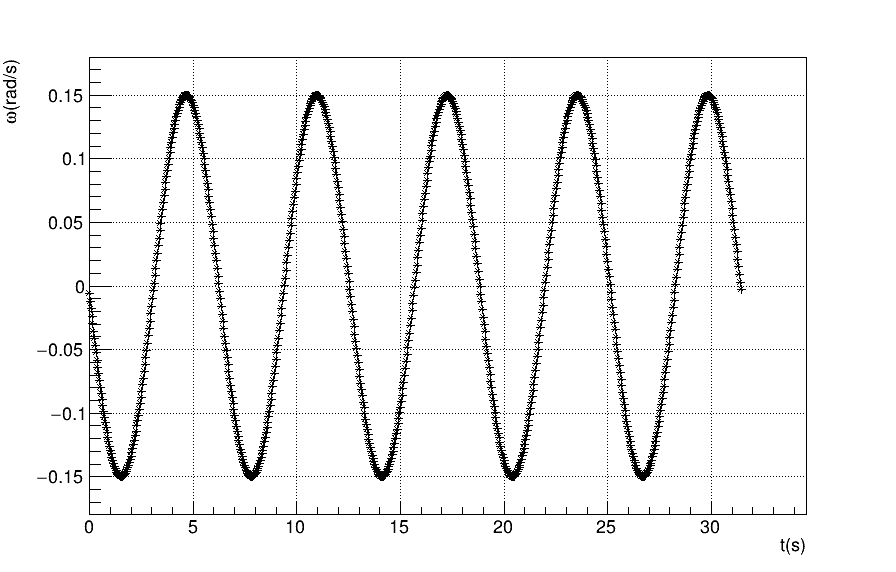
\includegraphics[scale=0.15]{../q1/plots/omega_t_RK.png}
        \captionof{figure}{Gráficos de $\omega \times t$ para os métodos de Euler simples, Euler-Crome e Runge-Kutta, respectivamente da esquerda para direita. }
    \end{center}
\item Os graficos abaixo mostra as sobreposições da energia cinética, potencial e total; onde fica clara a diferença entre cada um dos métodos, principalmente nos dois últimos.
    \begin{center}
        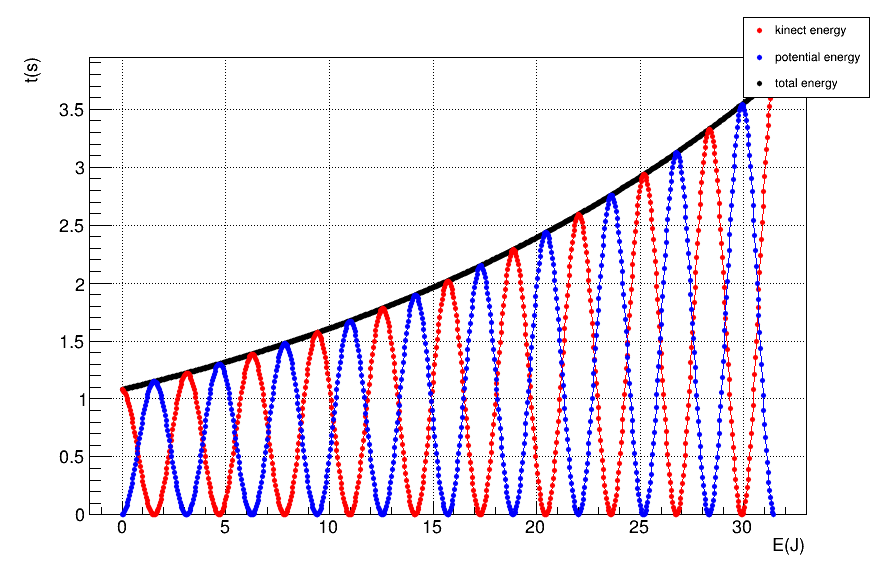
\includegraphics[scale=0.15]{../q1/plots/Energies_t_euler.png}
        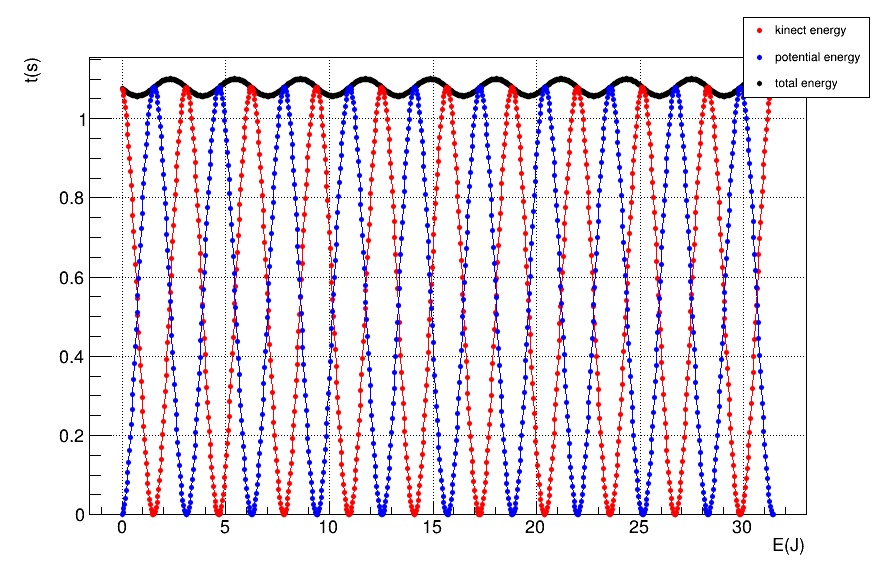
\includegraphics[scale=0.15]{../q1/plots/Energies_t_ec.png}
        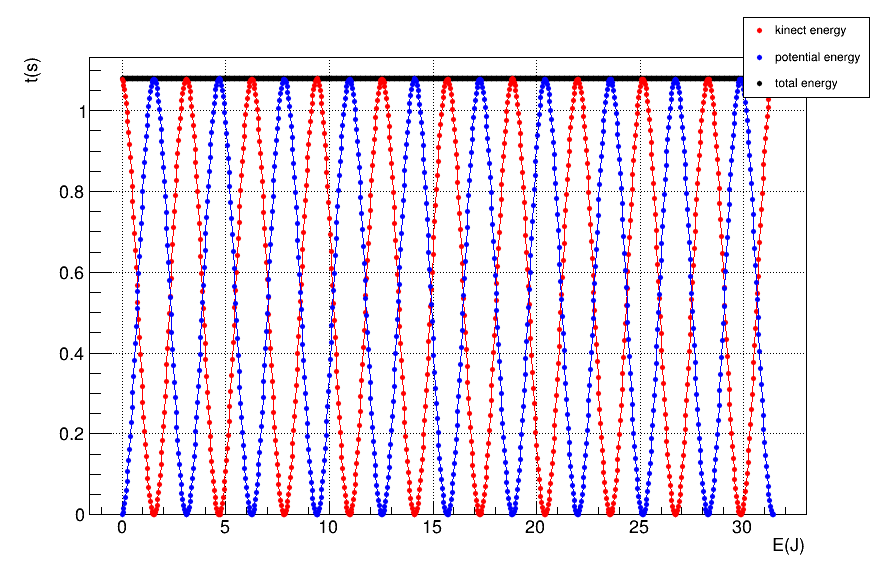
\includegraphics[scale=0.15]{../q1/plots/Energies_t_RK.png}
        \captionof{figure}{Gráficos das energias cinética, potencial e total em função do tempo para os métodos de Euler simples, Euler-Crome e Runge-Kutta, respectivamente da esquerda para direita. }
    \end{center}
    \item A partir do item (c) pode-se ver que o método de Euler simples não conserva a energia do sistema. Esta vai aumentando rapidamente. Já no método de Euler-Cromer, há uma melhora significativa que só pôde ser observada
    neste gráfico de energia. Embora a energia mecânica não esteja se conservando, ela está mudando com um comportamento oscilatório. Ou seja, a diferença nos gráficos de $\theta \times t$ e $\omega \times t$ é muito sútil.
    O impressionante deste método é que a única mudança em relação ao anterior, é que o $\theta$ é calculado com um passo a mais do $\omega$. O método de Runge-Kutta se mostra superior aos dois anteriores pois a energia total do sistema parece se conservar.
\end{enumerate}
\end{document}